
\section{Architektúry konvolučných neurónových sieti}
\label{sec:architekuraCNN}
Model ktorý bol zvolený je inšpirovaný architektúrov AlexNet (vid. \ref{subsec:popularCNN}).
Architektúra obsahuje celkovo 15 vrstiev z ktorých 4 sú konvolučné, 4 max pooling, 5 dropout vrstiev a 2 dense vrstvy.
Veľkosť vstupu do prvej vrstvy je 128x128 pixelov.
Vo všetkých konvolučných vrstvách boli použité filtre o veľkosti 2x2 s krokom 1 a bolo použité nulové zarovnanie
Každou vrstvou sa množstvo filtrov zdvojnásobuje, s počiatočných 16 až na 128 v poslednej vrstve.
Pooling vrstvy su typu max, veľkosť zhlukou je 2x2 pixely s posunom 2 do každej osi.
Za každou pooling vrstvou sa nachádza Droupout vrstva s nastavením 0.2, ciže 20 percent prepojení sa zahadzuje.

Po piatich skupinách konvolučnej, pooling a droupout vrstvy nasleduje dense vrstva s počtom prepojení 1024 a dropout vrstvou s nastavním 0.5.
Ako posledná je dense vrstva s 2 alebo 72 prepojeniami a softmax klasifikátorom, počet výstupov záleží či určujeme typ alebo náklon zbrane.
V celej sieti su použité ReLu aktivačné funkcie.

\begin{figure}[H]
    \centering
    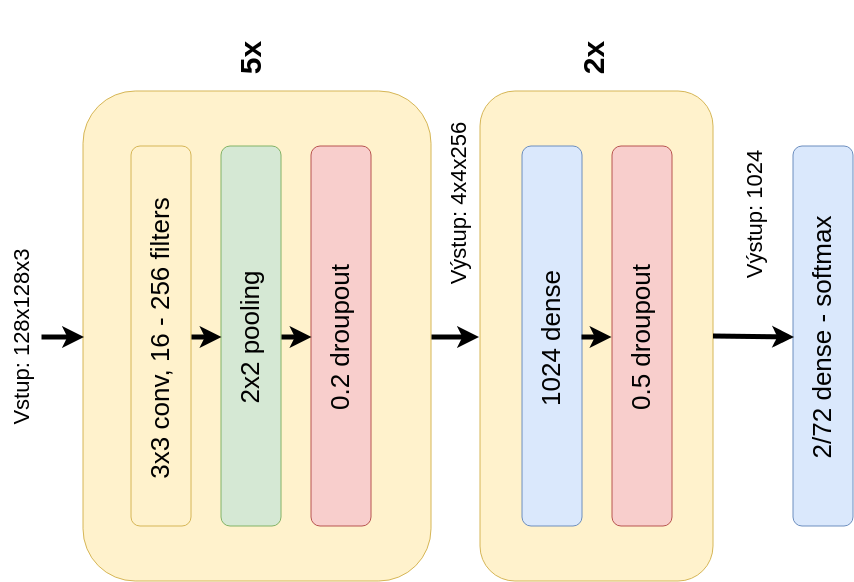
\includegraphics[width=0.6\textwidth]{AlexNet_Like}
    \caption{Architektúra opísanej siete.}
    \label{pic:kNN}
\end{figure}

Druhý navrhovaný model je inšpirovaný architektúrov VGG sieti (vid. \ref{subsec:popularCNN}).
Vzhľadom na možnosti výkonu na ktorom bude trénovanie prebiehať, je navrhovaná sieť o jeden blok vrstviev menšia a taktiež konvolučne vrstvy obsahujú menej filtrov.

Celkovo sieť obsahuje 2 bloky po 2 konvolučných vrstvách a pooling vrstve, 2 bloky po 3 konvolučných vrstvách a pooling vrstve a ako posledné
    sú 2 dense vrstvy s počtom prepojení 2048 a posledná výstupna vrstva s počtom prepojení 2 alebo 72 a softmax klasfikátorom.
Každá konvolučna vrstva obsahuje filtre o veľkosti 2x2, krokom 1 s použitím nulového doplnku.
Počty filtrov sa po blokoch zdvojnásobujú od 16 až po 256 filtrov.
Všetky vrstvy používajú ReLu aktivačnú funkciu.

\begin{figure}[H]
    \centering
    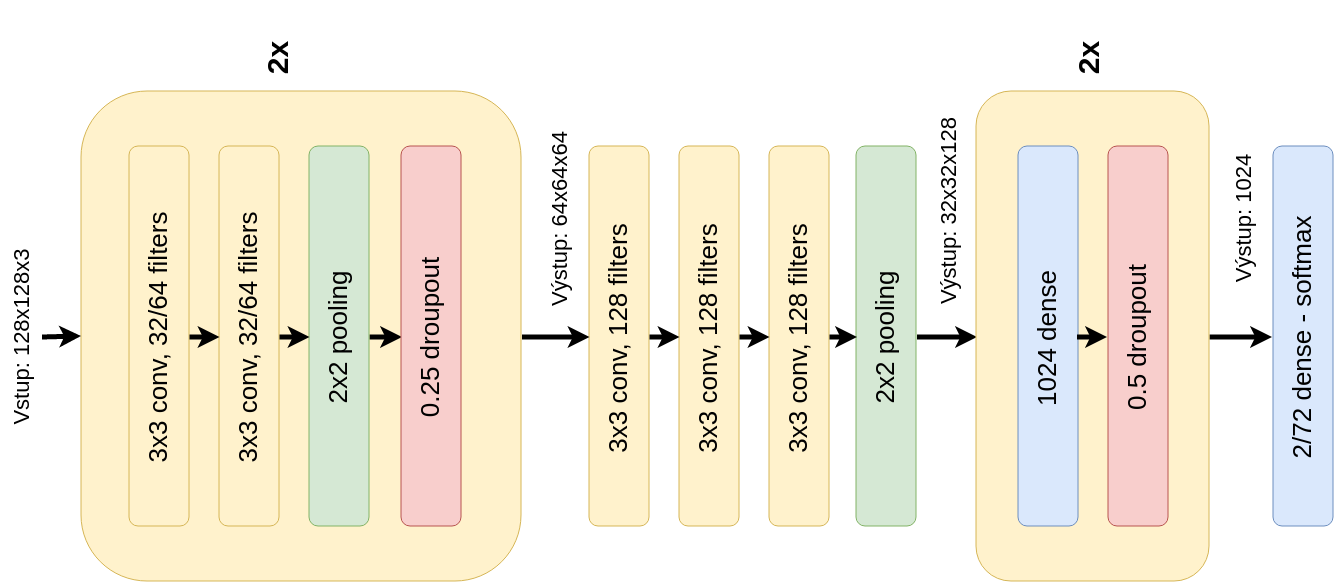
\includegraphics[width=0.8\textwidth]{VGG_Like}
    \caption{Architektúra opísanej siete.}
    \label{pic:kNN}
\end{figure}

\subsection{Hodnotenie presnosti siete}

\begin{comment}

    \begin{figure}[H]
        \centering
        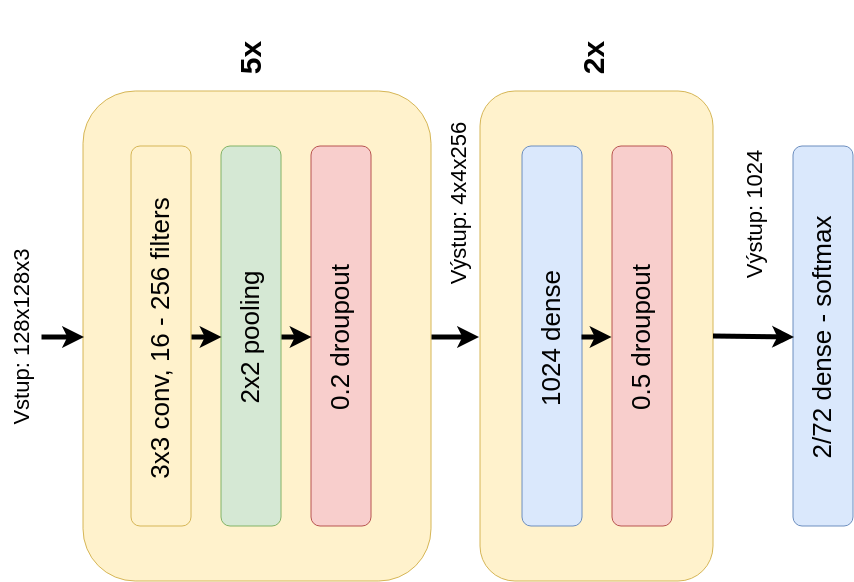
\includegraphics[width=0.32\textwidth]{AlexNet_Like}
        \caption{.}
        \label{pic:kNN}
    \end{figure}

    - Pridat ake optimalizatory a celkovo s akymi argumetmi spustat trenovanie, kolko epoch a pod...
    - Zdovodnovat preco prave taketo nastavenie konvolucnej siete.
    - pocet epoch bude potrebne zistit experimentalnych sposobom, alebo pouzit funkciu na save best of Keras-u

\end{comment}
